\section{Efficiency calculations}
Measurements of the total selection efficiencies
$\eff{tot}(\btokpipimumu)$,
$\eff{tot}(\btopsitwosk)$,
$\eff{tot}(\btophikmumu)$, and
$\eff{tot}(\btojpsiphik)$,
must be made in order to determine the branching fractions for the decays \btokpipimumu and
\btophikmumu.
These efficiencies were calculated using simulated events; therefore, in order that the above
efficiencies are correct it is imperitive that thesimulated events describe the data accurately.

There are some variables which are known to be poorly described in data, particularly track
multiplicity and the \chisqvtx of the \Bp candidate.
Track multiplicity is known to be poorly modeled by simulation, as can be seen in
\Fig{fig:hhh:ntracks}.


\begin{figure}
  \begin{center}
    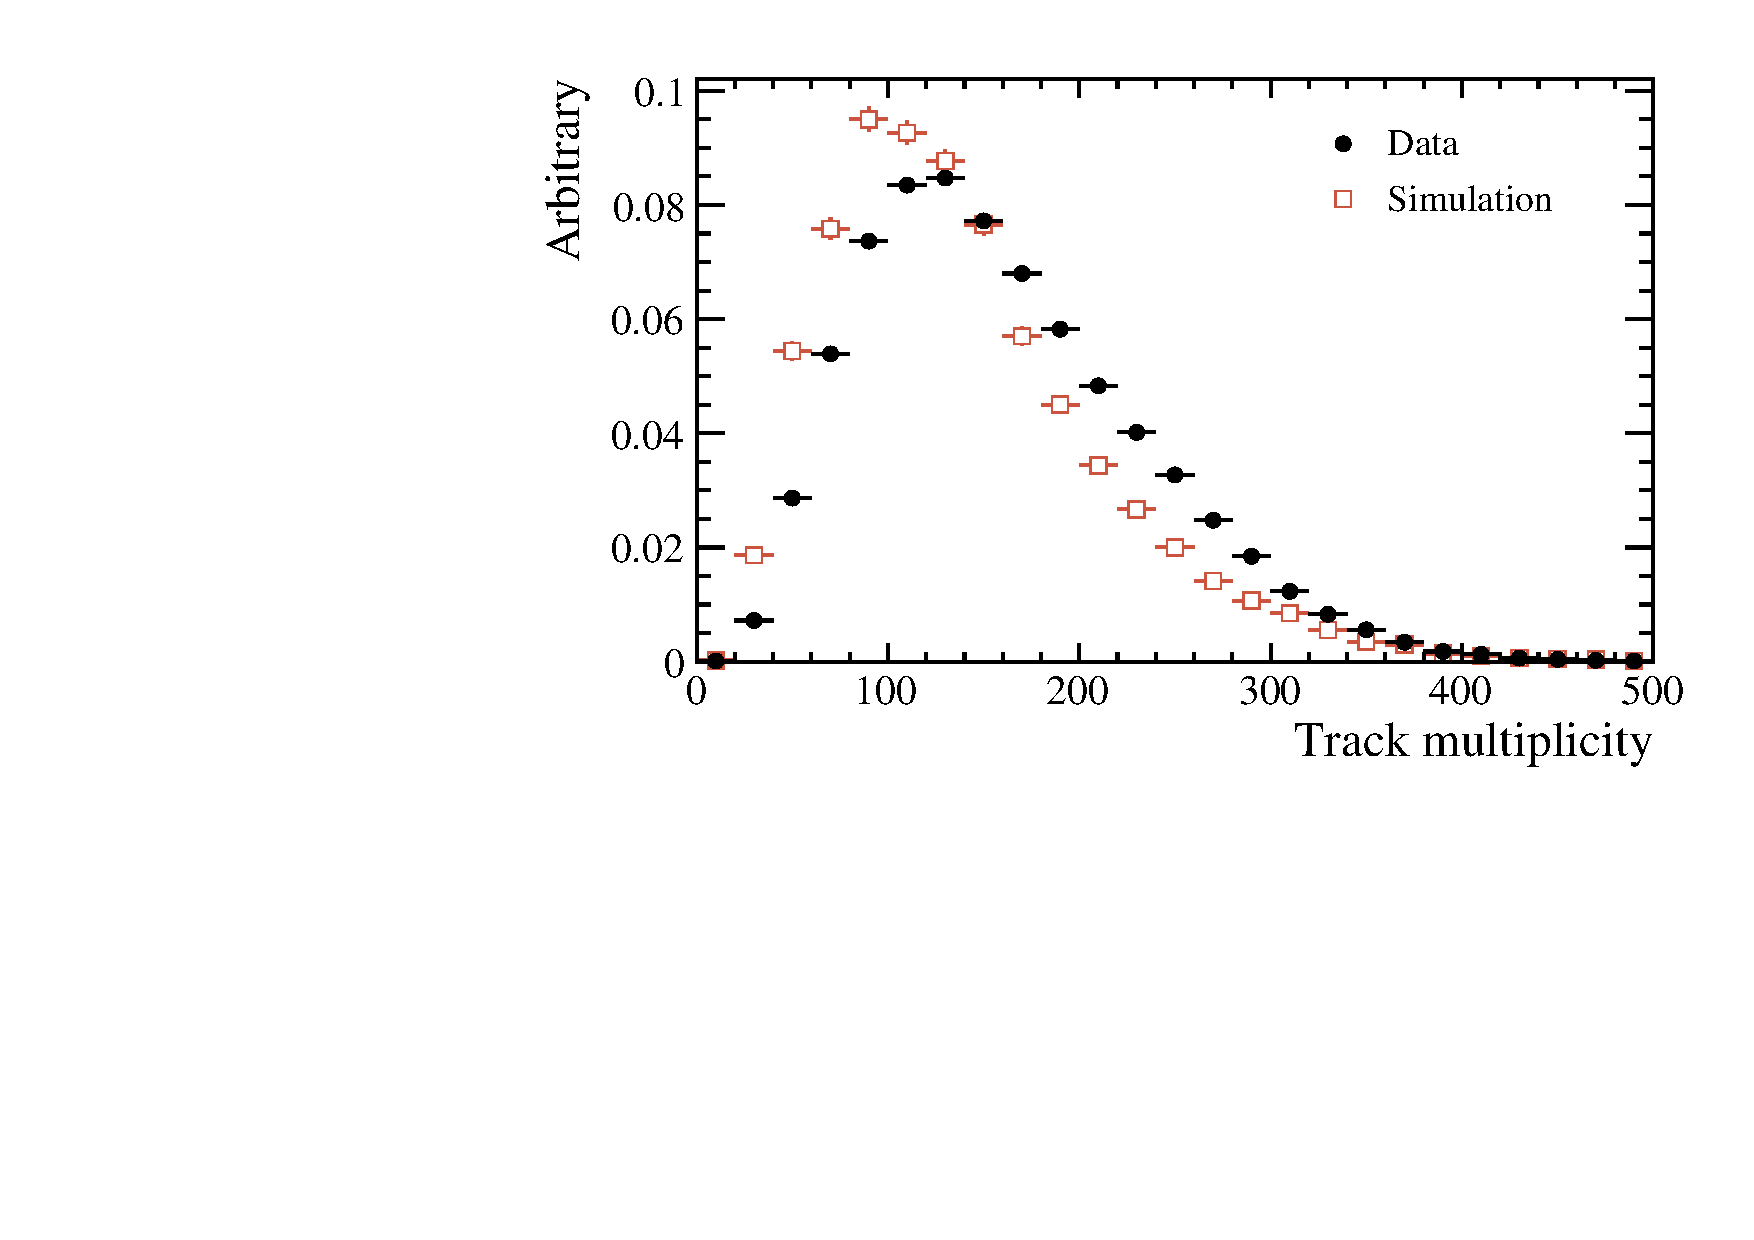
\includegraphics[width=0.48\textwidth]{ntracks}
    \caption{\small
      Distributions of track multiplicity for (black circles) data and (red squares) simulation.
      Simulated events are known to mis-model the track multiplicity, having a lower average number
      of tracks per event.
    }
    \label{fig:hhh:ntracks}
  \end{center}
\end{figure}






